% Define block styles
    
\tikzstyle{block} = [rectangle, draw=blue, drop shadow,very thick,top color=white,              % a shading that is white at the top...
    bottom color=blue!20!,%fill=blue!20, 
    text width=8.5em, text centered, rounded corners, minimum height=5em,node distance=4cm,]
 
 \tikzstyle{blockred} =  [rectangle, draw=red, drop shadow,very thick,top color=white,              % a shading that is white at the top...
    bottom color=red!20!,%fill=blue!20, 
    text width=8em, text centered, rounded corners, minimum height=5em,node distance=3cm,]
\tikzstyle{blockgreen} = [rectangle, draw=green, drop shadow,very thick,top color=white,              % a shading that is white at the top...
    bottom color=green!20!,%fill=blue!20, 
    text width=8em, text centered, rounded corners, minimum height=5em,node distance=3cm,]

\tikzstyle{blocksmall} = [rectangle, draw=blue, drop shadow,very thick,top color=white,              % a shading that is white at the top...
    bottom color=blue!20!,%fill=blue!20, 
    text width=2em, text centered, rounded corners, minimum height=2em,node distance=3cm,]
 

\tikzstyle{line} = [draw,line width=1.0pt, -latex']
\tikzstyle{dblarrow} = [thick,<->,shorten >=1pt,shorten <=1pt,>=stealth, -latex']
\tikzstyle{line2} = [thick,->,shorten >=1pt,shorten <=1pt,>=stealth, -latex']
    
\begin{tikzpicture}[node distance = 2cm, auto]
    % Place nodes
\node [block] 		(pc) {Computer\\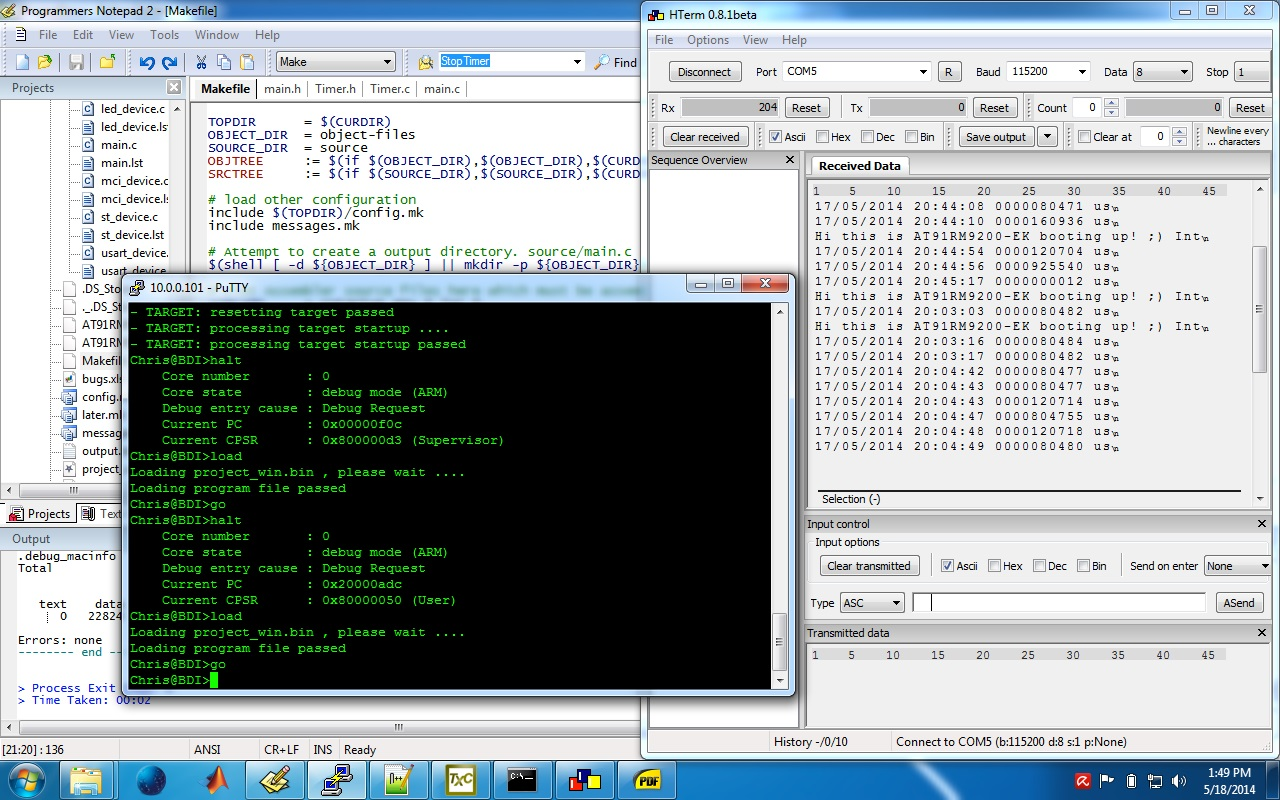
\includegraphics[height=4em]{images/IDE.jpg}};
\node [block, right of=pc, xshift=4cm] 		(BDI) {BDI2000\\ 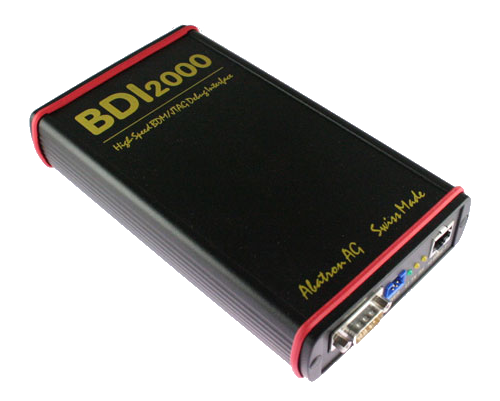
\includegraphics[height=4em]{images/bdi2000.png}};
\node [block, below of=pc] 		(IO) {Input Sensor\\ 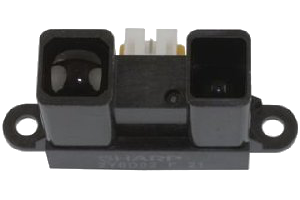
\includegraphics[height=4em]{images/GP2Y0D02YK0F.png}};
\node [block, below of=BDI] 		(AT) {AT91RM9200\\ 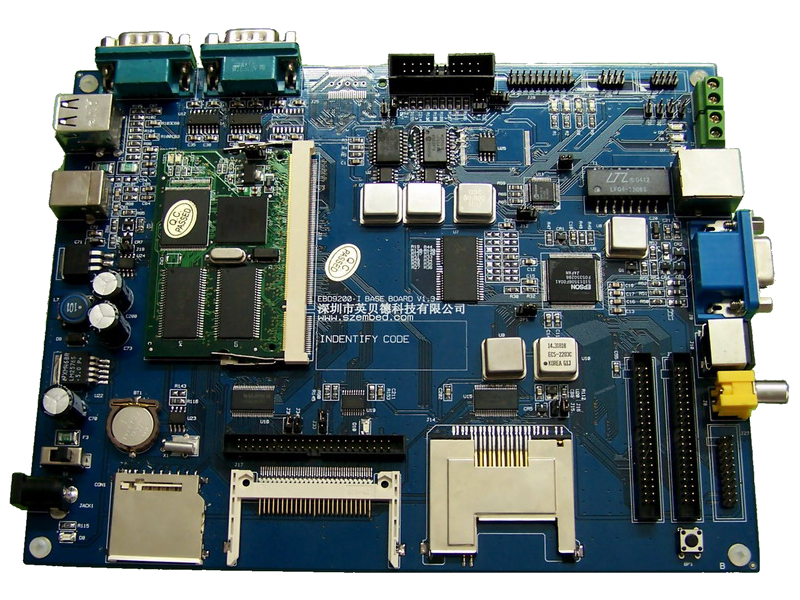
\includegraphics[height=4em]{images/AT91RM9200DB.png}};
%\node [block] 	(um2) {Umrechnung\\ SollTrq $\Rightarrow$ SollPos \\ };
%\node [block,  below of=abstmp] 	(tempmod) {$\Delta$-Temperatur- \\Algorithmus\\  };
%\node [blocksmall,  right of=tempmod, node distance=4cm] 	(multi) {$\times$};
%\node [blocksmall,  right of=multi, node distance=4cm] 	(multi2) {$\times$};
%\node [blocksmall,  above of=multi2] 	(divi) {$\div$};
%\node [blocksmall,  above of=divi] 	(minus) {$-$};
	%
 %
    %% Draw edges
    %\path [line] ([xshift=-2cm,yshift=+0.5cm] abstmp.west)--node [midway, above]{$Act_{Pwr}$}([yshift=+0.5cm] abstmp.west);
%\path [line] ([xshift=-2cm,yshift=-0.5cm] abstmp.west)--node [midway, above]{Tumg}([yshift=-0.5cm] abstmp.west);   
%
%
%\path [line] ([xshift=-2cm,yshift=+0.7cm] tempmod.west)--node [midway, above]{$P_{Eng\_Last}$}([yshift=+0.7cm] tempmod.west);
%\path [line] ([xshift=-2cm ] tempmod.west)--node [midway, above]{$nmot$}( tempmod.west);
%\path [line] ([xshift=-2cm,yshift=-0.7cm] tempmod.west)--node [midway, above]{vfzg}([yshift=-0.7cm] tempmod.west);   
%
%
\draw [dblarrow,<->] ([yshift=0.25cm]pc.east)--node [midway, above]{Ethernet, Telnet}([yshift=0.25cm]BDI.west);  
%\path [line] ([yshift=0.25cm]BDI.west)--node {}([yshift=0.25cm]pc.east);

\draw [dblarrow,<->] (BDI.south)--node [midway, right]{JTAG}(AT.north); 
%\path [line] (AT.north)--node {}(BDI.south); 

\draw [line2] ([yshift=-0.25cm]IO.east)--node [midway, below]{Digital Input}([yshift=-0.25cm]AT.west); 
\draw [dblarrow,<->] ([yshift=-0.25cm]pc.east)--([yshift=-0.25cm,xshift=2cm] pc.east)|-node [near start, above ,rotate=270]{\acs{UART}, RS232}([yshift=0.25cm] AT.west);
%\path [line] ([yshift=0.25cm]AT.west)-|([yshift=-0.25cm,xshift=2cm] pc.east)--([yshift=-0.25cm] pc.east);

%\path [line] ([xshift=-2cm] um2.west)--node [midway, above]{{SollTrq}}(um2.west); 
%\path [line] (abstmp.east)-|node [pos=0.27, above]{$Load_{Fact}$}( multi.north); 
%\path [line] (multi.east)--node [midway, above]{Gew. $\Delta T_{Hydr}$}( multi2.west);  
%\path [line] ([xshift=2cm] multi2.east)--node [midway, above]{$Vol_{Hyd1K}$}(multi2.east);
%\path [line] (multi2.north)--node [midway, above, rotate=90]{$\Delta Vol_{Hydr}$}(divi.south);
%\path [line] ([xshift=-2cm] divi.west)--node [midway, above]{{$Aktor_{Area}$}}(divi.west);   
%\path [line] (divi.north)--node [midway, above, rotate=90]{$Act_{Poscor}$}(minus.south);
%\path [line] (um2.east)--node [midway, above]{$SollPos$}(minus.west);
%\path [line] ( minus.east)--node [midway, above]{$SollPos_{Cor}$}([xshift=2cm] minus.east);
\end{tikzpicture}